\chapter{Organic Synthesis: Building and Route Planning}

\begin{kaichang}
Look in the medicine cabinet for aspirin: white tablets with the awkward name acetylsalicylic acid on the leaflet. Worldwide production is about forty thousand tonnes annually, enough to fill a dozen or so railway cars.

Now imagine willow-bark decoction, brownish yellow and bitter. Ancient Greeks drank it for fever and pain over two thousand years ago; ancient Chinese people also used willow branches to dispel heat.

Write a choice: if both reduce fever, which would you choose, and why? I suspect many would favor willow water as natural and presumably safer than a chemical-factory product.

At the end, revisit your answer. Natural versus synthetic points in the wrong direction from the outset. The real questions lie at molecular scale: which molecule, how was it made, and how much else was produced in making it?
\end{kaichang}

\section{Two Origins of a Tablet}

Begin with observable, measurable facts.

Crushed aspirin is a slightly sour white powder, almost insoluble in cold water. Willow decoction is bitter from compounds called salicins. Nineteenth-century chemists isolated salicin and found the body converts it to salicylic acid. This reduces fever and pain, but its strong acidity and stomach irritation make direct ingestion unpleasant.

Chemists performed small molecular surgery: put an acetyl cap on salicylic acid's hydroxyl, \chem{-OH}. The resulting acetylsalicylic acid is aspirin. The aim was straightforward, easier administration and better gastrointestinal tolerance. \textbf{The framework hardly changed}; the salicylic-acid skeleton remained the basis of its activity.

How is that surgery done? Given a target, how do chemists choose starting materials and the order of operations?

First remember one fact: Chapter 35's melting points, chromatography, and spectroscopy identify factory-made acetylsalicylic acid and the same compound theoretically prepared from natural starting materials as \textbf{the same molecule}. Molecules keep no diary and bear no sign of willow bark versus reactor origin. We will return to this.

\section{Learn to Take Apart before Building}

Your boss gives you acetylsalicylic acid as a target. What do you do?

The direct approach is trial: mix starting materials, heat, and hope. Some early nineteenth-century chemists did this, with success comparable to throwing parts into the air and expecting a watch to assemble on landing.

Later chemists learned to reverse direction: \textbf{take apart, then build}. Look at the target and ask what simpler fragments would result from cutting a bond. Can each fragment be cut again, until only cheap purchasable materials remain? Analysis runs backward; assembly forward. This systematic reverse thinking is \textbf{retrosynthetic analysis}, organized by American chemist Corey in the 1960s. He stressed that it is a learnable tool, not genius inspiration: a watch repairer first understands the blueprint, not turns screws.

\begin{center}
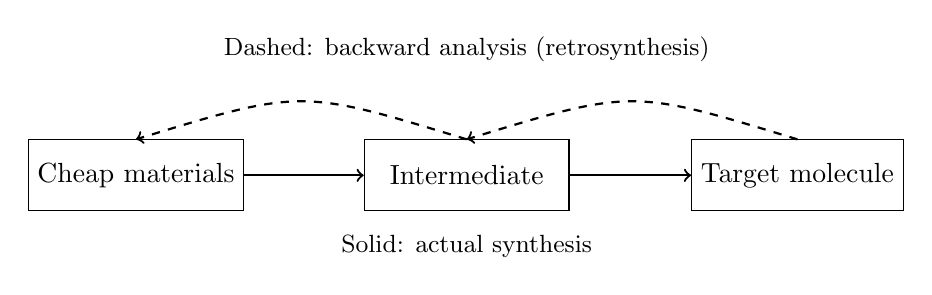
\begin{tikzpicture}[scale=1.0]
\node[draw,rectangle,minimum width=2.6cm,minimum height=0.9cm] (a) at (0,0) {Cheap materials};
\node[draw,rectangle,minimum width=2.6cm,minimum height=0.9cm] (b) at (4.2,0) {Intermediate};
\node[draw,rectangle,minimum width=2.6cm,minimum height=0.9cm] (c) at (8.4,0) {Target molecule};
\draw[->,thick] (a) -- (b);
\draw[->,thick] (b) -- (c);
\draw[->,dashed,thick] (c.north) .. controls (6.3,1.1) .. (b.north);
\draw[->,dashed,thick] (b.north) .. controls (2.1,1.1) .. (a.north);
\node at (4.2,-0.9) {\small Solid: actual synthesis};
\node at (4.2,1.6) {\small Dashed: backward analysis (retrosynthesis)};
\end{tikzpicture}
\end{center}

This human-made diagram organizes thinking; boxes and arrows do not depict real molecules.

Practice on aspirin. Acetylsalicylic acid contains an ester, Chapter 40's acid--alcohol handshake. Make the first retrosynthetic cut there, yielding salicylic acid and a small acetyl donor. Salicylic acid is purchasable; acetic anhydride supplies acetyl, roughly two acetic acids minus water. Both are cheap and available, so the whole blueprint is dismantled in one layer.

Most drugs are much more complex, needing a dozen or dozens of layers, an upside-down tree rather than a line. The principle is identical: cut only bonds that can also be rejoined.

\section{Three Questions of Where}

A blueprint is only the beginning. Real molecules have several reactive sites, like multiple solder points on a circuit board. Each operation must answer three questions:

\begin{itemize}[itemsep=2pt]
\item \textbf{Where does reaction occur?} With several Chapter 37 groups, why should a reagent touch only one? This is chemoselectivity. Salicylic acid has both hydroxyl and carboxyl; acetylation should affect only hydroxyl, while the wrong reagent may involve carboxyl too.
\item \textbf{Where does reaction stop?} Chapter 40 oxidized alcohol to aldehyde and onward to acid. Want aldehyde? Brake midway with a mild oxidizer or remove aldehyde immediately as it forms.
\item \textbf{Which spatial structure forms?} Chapter 42's mirror hands can have very different drug effects. New chiral centers often form both hands; how can the desired one dominate?
\end{itemize}

Poor answers defeat beautiful plans. Chemists devised a simple but effective fallback: \textbf{protecting groups}.

To paint a wall without painting its switch plate, mask the plate, paint, then peel off the tape. Protecting groups are molecular masking tape. If A must react while B must not, cap B first, work on A, then remove the cap.

Costs are obvious: protection and deprotection add two reactions, consume materials, create waste, and reduce yield. Protecting groups are necessary waste, avoided whenever possible. Naturally selective reagents could remove the necessity. Remember that seed for the chapter's end.

\section{Every Step Charges a Toll}

Now money---or rather, yield. No reaction converts with absolute perfection: some starting material remains, and isolation loses some product. Each step's recovered fraction is yield.

Ten steps at a respectable $90\%$ each: what overall yield? Intuition may say roughly ninety percent, but calculate:

\[0.9^{10}\approx 0.35\]

Only thirty-five percent remains. A hundred grams in gives thirty-five grams out, with sixty-five paid in tolls. Multistep synthesis has harsh mathematics: \textbf{yields multiply}, each loss compounding later ones. Twenty steps gives $0.9^{20}\approx 0.12$, wasting more than eighty percent.

\begin{qiaoliang}
Beyond yield is \textbf{atom economy}: not how much product was recovered, but how many reactant atoms end up in the desired molecule. Calculate target molar mass divided by the sum of reactant molar masses.

For aspirin, salicylic acid, \chem{C_7H_6O_3}, \ud{138}{g\cdot mol^{-1}}, reacts with acetic anhydride, \chem{C_4H_6O_3}, \ud{102}{g\cdot mol^{-1}}, to make acetylsalicylic acid, \chem{C_9H_8O_4}, \ud{180}{g\cdot mol^{-1}}, and acetic acid, \ud{60}{g\cdot mol^{-1}}:

\[\text{Atom economy}=\frac{180}{138+102}=\frac{180}{240}=75\%\]

Even at perfect $100\%$ yield, a quarter of entering atoms must become acetic-acid byproduct. Atom economy is a route's inherited constitution, yield its performance: a poor constitution imposes a waste limit however well performed. Green chemistry begins here, choosing low-waste blueprints instead of treating waste afterward. Chapter 38's additions joining two molecules without byproducts naturally have $100\%$ atom economy and are designers' favorites.
\end{qiaoliang}

\begin{shiyan}
\textbf{Simulate Ten-Step Synthesis with Dice} (paper simulation, no chemicals).

Materials: a die, paper, and pen.

Procedure: suppose each of ten steps yields five-sixths, about $83\%$. Rolls 1–5 succeed; 6 fails and scraps the batch. Start at Step 1; ten consecutive successes deliver final product. Any 6 means restart.

What to observe: play twenty rounds and count completions. Theoretical success is $(5/6)^{10}\approx 16\%$, about three rounds in twenty. Was yours close? Now allow one reroll of 6, failing only on a second 6, making success $35/36$, about $97\%$. Experience how small per-step improvements transform the whole route.

Safety: paper, pen, and die present no chemical danger. Real synthesis uses toxic solvents, corrosive reagents, and hot glassware. \textbf{Never imitate actual synthesis at home}. For reactors, use reputable educational videos or wait for a teacher's demonstration.
\end{shiyan}

Yield and atom economy illuminate industrial choices. Ibuprofen, a later painkiller than salicylic acid, is classic: an older six-step route had about $40\%$ atom economy; a 1990s three-step process reached about $77\%$, nearly $99\%$ counting reused byproducts. It more than halved waste and won a green-chemistry award. Smarter route design, not harsher conditions, was the secret and this chapter's theme.

\section{The Reaction Equation Arrives}

We deliberately delayed the equation. Now write aspirin's step:

\[\chem{C_7H_6O_3} + \chem{C_4H_6O_3} \rightarrow \chem{C_9H_8O_4} + \chem{C_2H_4O_2}\]

Salicylic acid plus acetic anhydride makes aspirin plus one acetic acid. Equal carbon, hydrogen, and oxygen counts uphold atom conservation (Chapter 24). Behind the line stands every discussion: retrosynthesis chooses ingredients, selectivity chooses hydroxyl, and atom economy identifies unavoidable acetic-acid byproduct.

Read the arrow not as magic but as the statistical result of many molecules rearranging through Chapter 38's electron-pair mechanisms. Chapter 27's energy rules constrain direction; Chapter 28's rate rules constrain speed. Blueprint, energy, and rate are all indispensable.

\section{Mold to Antibiotics: A Century-Long Relay}

Aspirin's one step is too simple to show route planning's full power. Take a harder story.

\begin{zhengju}
In 1928, London bacteriologist Fleming returned from holiday to an odd mold-contaminated dish: staphylococci did not grow around blue-green mold. Perhaps mold consumed their nutrients, a reasonable alternative. He filtered mold-grown liquid, \textbf{removing all living mold}, yet it still killed bacteria. This excluded nutrient competition and indicated a secreted bactericidal substance, which he named penicillin.

He then stalled. Penicillin was unstable, difficult to purify, and too dilute for treatment. He even thought it might serve only as a topical disinfectant. Discovery was not usability; manufacturing routes had to bridge the gap.

Ten years later, Florey and Chain's Oxford team used techniques including freeze-drying for purer penicillin. In the famous 1940 experiment, eight mice received lethal bacteria: four treated survived, all four untreated died. Strong evidence, but treating one person required extraction from hundreds of liters of culture. Wartime demand drove discovery of a higher-yielding strain on moldy cantaloupe and deep-tank fermentation. \textbf{Letting mold do the synthesis labor} raised output hundreds to thousands of times.

The final mystery was structure. Chemists disputed candidates for years until Hodgkin's 1945 X-ray crystallography, one of Chapter 35's detective methods, settled a strained four-membered $\beta$-lactam ring. Its weakness became clear: acid and bacterial enzymes readily opened it. In the late 1950s, scientists isolated the side-chain-free core directly from fermentation broth, then chemically fitted new side chains for acid resistance, broader antibacterial action, or resistance to bacterial enzymes. Semisynthetic penicillins emerged from blueprints and still save lives.

Review the relay: observation, exclusion, purification, quantitative evidence, fermentation scale-up, structure determination, molecular modification. No step was a lone genius's performance; each asked where molecules come from and how to make more, better, and more suitable ones.
\end{zhengju}

Notice one detail: penicillin still is not manufactured by total synthesis, building the whole molecule from simple ingredients. Chemists can do it, accomplished in 1964, but long, expensive, low-yield routes lose to mold building the chassis and chemists furnishing it. This leads directly to blueprint thinking's limits.

\section{A Drawing Is Not a Buildable Route}

Retrosynthesis is a remarkable map, not a road. Four boundaries stand out:

\begin{itemize}[itemsep=2pt]
\item \textbf{Bonds cut on paper may not re-form in a flask}. Analysis locates cuts, not whether fragments truly meet and bond. Every step must pass energy feasibility (Chapter 27) and kinetic barriers and side reactions (Chapter 28).
\item \textbf{Step count is an enemy}. Compounded yields make dozens or hundreds of steps for complex natural molecules often yield less than one percent. Total vitamin \chem{B_{12}} synthesis took two teams, almost a hundred people, and eleven years, proving capability rather than sensible production. Commercial \chem{B_{12}} comes from fermentation.
\item \textbf{A route map does not identify the cheapest path}. Candidates require comparing yield, atom economy, ingredient price, waste treatment, and safety: engineering and economics beyond the drawing.
\item \textbf{Some selectivity is almost insoluble}. Reagents often cannot select the desired site or hand, forcing protecting groups or resolution that discards half the product. This traditional synthesis pain is the closing seed's origin.
\end{itemize}

Do not confuse drawing a retrosynthetic tree with feasibility. Plans begin thought; experiments establish practicality. Good synthetic chemists spend half their time drawing and half learning reality at the flask.

\begin{wuqu}
``Natural is safe; synthetic is harmful.'' This label most needs dismantling.

Counterexamples attack both sides. Ricin, aconitine, and death-cap amatoxins are entirely natural and exceptionally poisonous; natural salicylic acid still irritates stomachs. Conversely, synthetic insulin and antibiotics save millions yearly. Factory vitamin \chem{C} in effervescent tablets and plant-made vitamin \chem{C} in lemons are \textbf{the same molecule}, identical structure and properties, with no instrument able to distinguish origin.

Toxicity depends on \textbf{the molecule and dose}, not origin, as Chapter 35 distinguished detection from harm. Calling natural good and synthetic bad resembles judging character by clothing's manufacturing country: convenient, and truly wrong.
\end{wuqu}

\section{Back to the Aspirin Pack}

Now answer: willow decoction or aspirin?

The right response is that the question started wrongly. Active ingredients are molecules, not origins. Willow's problem is \textbf{uncertain composition and uncontrolled dose}: salicin varies among trees and boiling durations, leaving unknown active amounts and untested impurities per cup. Aspirin's advantage is \textbf{known composition, standardized purity, and precise dose}, not synthesis itself. Route design, purification, and quality control make molecular types and numbers per tablet definite.

Tell the whole truth too: aspirin has side effects, including gastrointestinal irritation, greater bleeding risk, and rare serious risks in children after certain viral infections. Whether and how much to use belongs to doctors and instructions considering individual differences. This book prescribes nothing. Scientific honesty neither worships nature nor glorifies tablets.

Parallel everyday examples include mostly synthetic ice-cream vanillin, identical to vanilla pods' main aroma molecule, and jeans' indigo, formerly plant-extracted and now almost entirely synthetic, with unchanged dye molecules. Price, flavor complexity, and environmental cost can reasonably favor either origin. Natural-is-safe and synthetic-is-harmful cannot.

\section{Cells: Master Synthesizers without Flasks}

Remember the difficulty of selecting one site or hand without protective masking?

Here is an uncomfortable fact: every cell is synthesizing right now, better than any chemist. At $37\,^{\circ}\mathrm{C}$, ordinary pressure, and in water, cells make proteins, fats, and sugars, choosing any desired group among dozens, never getting handedness wrong, without organic solvent or protecting groups, and almost no waste.

How? Protein molecular machine tools, enzymes, hold substrates at exact angles and positions, permitting reaction \textbf{only} at the chosen site and stereochemistry. Chemists' dream selectivity is enzymes' daily routine. Industry has already surrendered and learned: semisynthetic penicillin joins cellular chassis-building with human route design.

But why do enzymes recognize positions? Where does cellular energy come from, and who supplies blueprints? These go beyond organic chemistry into the next part. Part VI begins with life's chemical-system identity in Chapter 45, then sugars, fats, proteins, and enzymes in Chapter 49. Life solved selectivity through proteins and evolution billions of years before it gave chemists headaches.

\begin{tiaozhan}
Want a deeper calculation? Skipping leaves the thread intact. Ten linear steps at $90\%$ yield only $0.9^{10}\approx 35\%$. What if the target splits into comparable fragments, \textbf{two five-step branches followed by one joining step}? Each gives $0.9^5\approx 59\%$, then final joining multiplies by $90\%$: $0.9^5\times 0.9\approx 53\%$. Same ten steps and per-step yield, but overall yield rises from $35\%$ to $53\%$. A linear Step8 failure wastes seven steps' accumulated material; a failed branch only needs that branch remade. This is \textbf{convergent synthesis}, route design's second major tool after reducing steps. Real drugs are deliberately split into comparable fragments for this mathematical benefit. Test three branches of 3+3+4 steps before joining: higher or lower total yield?
\end{tiaozhan}

\section*{Try It Yourself}

\begin{sikaoti}
\item Chapter40 joined acid and alcohol into ester and water. Retrosynthetically cut ethyl acetate, \chem{CH_3COOCH_2CH_3}, found in polish solvent and fruit aromas. Mark the ester bond and first cut, name two starting materials, and draw solid synthesis arrows and dashed backward arrows.
\item An eight-step drug route yields $80\%$ per step. Calculate total yield and approximate starting mass for \ud{100}{g} final product, assuming similar molar masses. What does this make you think about steps?
\item What is atom economy for Chapter38's two-reactant, one-product, no-byproduct addition? Can substitution, one group replacing another, reach $100\%$? Why?
\item Diagram protecting-group costs: starting A with two groups, protective cap, reaction, cap removal, product. Mark possible material-loss exits at every arrow. Why necessary waste: what is necessary, what wasted?
\item Factory vitamin \chem{C} tablets and plant-made orange vitamin \chem{C}: the same molecule? Different water solubility or bodily absorption mechanisms? Explain molecules not remembering origin, then locate the error in better-absorbed natural-vitamin advertising.
\item You want an alcohol oxidized to aldehyde, but it continues to acid (Chapter40). Propose at least two ways to stop at the intended stage, explaining each principle.
\end{sikaoti}
